\subsection{Scope-Prune-Update for Single Edge Updates}

\begin{figure}
    \centering

    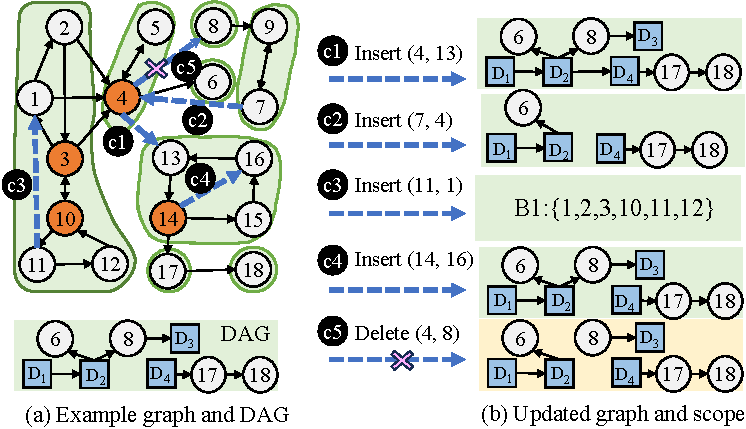
\includegraphics[width=1\linewidth]{figures/update_scope-crop.pdf}
    \caption{Five scope cases (\circled{c1}--\circled{c5}) for a single edge update on the running example.
    Cases \circled{c1}--\circled{c4} cover insertions classified by the structural relationship between the two endpoints; \circled{c5} covers deletion, classified by whether the removed edge is a bridge and at which GIR layer.
    Affected DAG nodes are highlighted in blue; yellow shading indicates a WCC split.}
    \label{fig:scope-update}
\end{figure}

We focus on \textit{single edge update} (insertion/deletion), as node insertions without edges do not affect connectivity and node deletions reduce to bulk edge deletions.
SPU processes each edge update in three steps: \textit{Scope} (classify the update and identify affected layers), \textit{Prune} (restrict the computation to the smallest affected region), and \textit{Update} (perform localized structural repair).

The central challenge is determining which GIR layers are affected by each operation.
Because GIR stores component labels, SCC membership, DAG ranks, and articulation-point metadata for every vertex, this classification requires no graph traversal.
As illustrated in Figure~\ref{fig:scope-update}, every edge update falls into one of five cases:
\circled{c1}~$s$ and $t$ reside in \emph{different WCCs} (insertion);
\circled{c2}~$s$ and $t$ reside in the \emph{same WCC but different SCCs} (insertion);
\circled{c3}~$s$ and $t$ reside in the \emph{same SCC but different BiCCs} (insertion);
\circled{c4}~$s$ and $t$ reside in the \emph{same BiCC} (insertion);
\circled{c5}~edge \emph{deletion}, whose scope depends on bridge status.

We now walk through each case.
For every case, we describe the scope decision (which layers are affected), the pruned region (what subgraph is examined), and the update action (how GIR is repaired).

\textbf{Case 1 (Insertion): $s$ and $t$ belong to different WCCs.}
The inserted edge connects two previously disconnected regions.
No directed cycle can form across WCC boundaries.
No articulation structure inside either component changes.

\textit{Scope.} Confined to the WCC layer only.

\textit{Prune and Update.} The two components are merged with an $O(1)$ label update.
Neither the SCC condensation DAGs nor the BC trees are touched.

\textit{Example.}
Inserting edge $(4,\,13)$ (\circled{c1}) bridges $\text{WCC}_1 = \{1\text{--}12\}$ and $\text{WCC}_2 = \{13\text{--}18\}$.
The two condensation DAGs are concatenated into a single one, as shown in Figure~\ref{fig:scope-update} (\circled{c1}).

\begin{figure}[t]
    \centering

    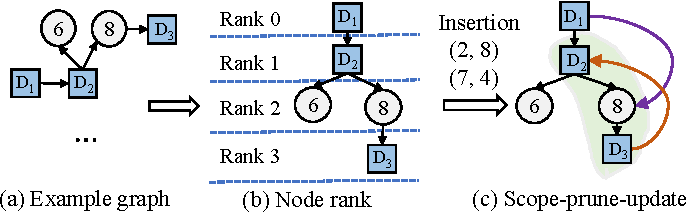
\includegraphics[width=1\linewidth]{figures/scope_update-crop.pdf}
    \caption{Rank-interval pruning for Case \circled{c2} (inter-SCC insertion). Each SCC is assigned a topological rank in the condensation DAG. When an inserted edge goes against the DAG order from $\mathrm{SCC}(s)$ to $\mathrm{SCC}(t)$, cycle detection is confined to the rank interval $[\mathrm{rank}(\mathrm{SCC}(t)),\,\mathrm{rank}(\mathrm{SCC}(s))]$ (shaded region), avoiding a global DAG traversal.}
    \label{fig:rank-prune}
\end{figure}

\textbf{Case 2 (Insertion): $s$ and $t$ are in the same WCC but different SCCs.}
The inserted edge $s \to t$ introduces a new arc between two SCC supernodes in the condensation DAG.
The critical question is whether this arc creates a directed cycle, which would cause two or more SCCs to merge.

\textit{Scope.} To answer this without traversing the entire DAG, GIR assigns each SCC a \emph{rank}, a compact topological index maintained incrementally alongside the condensation DAG.
If $\mathrm{rank}(\mathrm{SCC}(s)) < \mathrm{rank}(\mathrm{SCC}(t))$, the edge follows the existing DAG order and cannot close a cycle; the scope is limited to inserting a new DAG arc with no SCC-level structural change.
If $\mathrm{rank}(\mathrm{SCC}(s)) > \mathrm{rank}(\mathrm{SCC}(t))$, the edge goes against the DAG order and may introduce a cycle.
The scope then expands to the SCC and BiCC layers.

\textit{Prune.} As illustrated in Figure~\ref{fig:rank-prune}, GIR restricts cycle detection to the rank interval $[\mathrm{rank}(\mathrm{SCC}(t)),\,\mathrm{rank}(\mathrm{SCC}(s))]$ in the condensation DAG, avoiding a global DAG search.

\textit{Update.} If a cycle is confirmed within this interval, all SCCs on the cycle are merged, the condensation DAG is updated locally, and the BC trees of the affected SCCs are reconstructed.

\textit{Example.}
Inserting edge $(5,\,2)$ (\circled{c2}): vertex $5 \in D_2$ and vertex $2 \in D_1$, with $\mathrm{rank}(D_2) > \mathrm{rank}(D_1)$ because $D_1 \to D_2$ in the original DAG.
The edge goes against the DAG direction, so GIR runs cycle detection restricted to the interval $[\mathrm{rank}(D_1),\,\mathrm{rank}(D_2)]$ (Figure~\ref{fig:rank-prune}).
A cycle is confirmed; $D_1$ and $D_2$ are merged, and the BC tree within the new combined SCC is updated, as shown in Figure~\ref{fig:scope-update} (\circled{c2}).

\textbf{Case 3 (Insertion): $s$ and $t$ are in the same SCC but different BiCCs.}
Both endpoints lie within the same SCC, so no WCC or SCC membership can change.

\textit{Scope.} Confined to the BiCC layer: specifically, only the two BiCC blocks containing $s$ and $t$ are potentially affected.

\textit{Prune and Update.} The new edge may merge the two blocks into a single larger BiCC, eliminating one or more articulation points and updating the BC tree accordingly.

\textit{Example.}
Inserting edge $(11,\,1)$ (\circled{c3}): vertex $11$ is in block $b_1 = \{10,\,11,\,12\}$ and vertex $1$ is in block $b_2 = \{1,\,2,\,3\}$, both within $D_1$.
The two blocks merge into $b_1 = \{1,\,2,\,3,\,10,\,11,\,12\}$, as shown in Figure~\ref{fig:scope-update} (\circled{c3}).

\textbf{Case 4 (Insertion): $s$ and $t$ are in the same BiCC.}
Both endpoints already belong to the same biconnected component.
Adding an edge within an already 2-edge-connected subgraph cannot create new articulation points, split any BiCC block, or alter SCC or WCC structure.

\textit{Scope.} The update is a structural no-op for all GIR layers; no maintenance is needed.

\textit{Example.}
Inserting edge $(14,\,16)$ (\circled{c4}): both vertices lie in the same BiCC block of $D_4$, so the GIR remains unchanged (Figure~\ref{fig:scope-update}, \circled{c4}).

\textbf{Case 5 (Deletion):}
A \emph{bridge} is an edge whose removal disconnects the subgraph that contains it---formally, an edge $(s,\,t)$ is a bridge if and only if no alternative undirected path connects $s$ and $t$ after its removal.
Bridges are precisely the edges that do \emph{not} belong to any BiCC block of size $\geq 2$; GIR records this status directly, so bridge detection requires no traversal.
The scope of a deletion is determined by where in the GIR hierarchy the bridge sits.

\emph{Case 5a (non-bridge):}
The deleted edge belongs to a BiCC block with at least one alternative path between $s$ and $t$, so no component splits at any level.

\textit{Scope.} Confined to the BiCC layer: the removed edge may change block boundaries or articulation-point status within the enclosing SCC, but the change does not propagate upward.

\textit{Update.} GIR checks whether any articulation points have changed and repairs the BC tree locally.

\emph{Case 5b (bridge within an SCC):}
The deleted edge is a bridge, and both endpoints belong to the same SCC.
Its removal severs the unique undirected path between $s$ and $t$ inside that SCC, which may cause the SCC to split into two or more SCCs.

\textit{Scope.} Expands to the SCC layer: GIR checks whether the directed SCC breaks apart and, if so, partitions it, rebuilds the affected fragment of the condensation DAG, and reconstructs the BC trees of the resulting components.

\emph{Case 5c (bridge in the condensation DAG):}
The deleted edge is an inter-SCC arc and the only undirected path between two regions of the WCC.
Its removal disconnects the WCC entirely.

\textit{Scope.} Spans the WCC and BiCC layers: the WCC splits into two independent components, the condensation DAG is partitioned accordingly, and the BC trees on each side are updated.

\textit{Example.}
Deleting edge $(4,\,8)$ (\circled{c5}): this edge is a bridge because it is the sole undirected path between the $\{D_1, D_2\}$ side and the $\{D_3\}$ side of the WCC (Case~5c).
Its deletion splits the WCC into two components, as shown in Figure~\ref{fig:scope-update} (\circled{c5}), requiring WCC relabeling and BC tree updates on each resulting component.

\begin{table}[t]
    \centering
    \small
    \setlength{\tabcolsep}{4pt}
    \renewcommand{\arraystretch}{1.1}
    \caption{Scope rules for single edge update, organized by the five cases.}
    \begin{tabular}{c l l l}
    \toprule
    \textbf{Case} & \textbf{Endpoint relation} & \textbf{Op} & \textbf{Layers affected} \\
    \midrule
    1 & Different WCCs                & Insert & WCC only\\
    2 & Same WCC, different SCCs & Insert & SCC + BiCC\\
    3 & Same SCC, different BiCCs & Insert & BiCC only\\
    4 & Same BiCC                     & Insert & BiCC only\\
    \midrule
    5a & Non-bridge            & Delete & BiCC only \\
    5b & Bridge within SCC        & Delete & SCC + BiCC \\
    5c & Bridge in DAG            & Delete & WCC + BiCC \\
    \bottomrule
    \end{tabular}
    \label{tab:updates}
\end{table}

Table~\ref{tab:updates} summarizes the scope rules for all five cases.
Case~4 is a complete no-op: no GIR layer requires any maintenance.
For all other cases, the prune step restricts the computation to the smallest affected region, and the update step performs localized structural repair.
This three-step discipline ensures that SPU never performs more work than the structural change requires.
